\documentclass[tikz,border=2pt]{standalone}

\usepackage{pgfplots}
\pgfplotsset{compat=1.18}

\begin{document}
	
	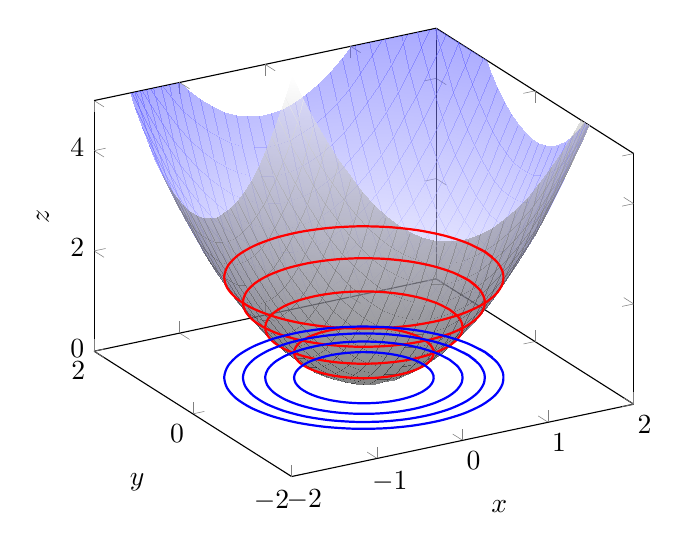
\begin{tikzpicture}
		\begin{axis}[
			view={-30}{30},
			domain=-2:2,
			y domain=-2:2,
			zmin=0, zmax=5,
			xlabel={$x$},
			ylabel={$y$},
			zlabel={$z$},
			mesh/interior colormap=
			{bluewhite}{color=(white) color=(blue)},
			colormap/blackwhite,
			]
			
			% Plotting the 3D surface
			\addplot3[surf, shader=interp, samples=30, opacity=0.5] {x^2 + y^2};
			
			% Plotting the level curves on the 3D surface
			\foreach \k in {0.5, 1, 1.5, 2} {
				\addplot3[domain=0:2*pi, samples=30, smooth, thick, color=red] ({sqrt(\k)*cos(deg(x))}, {sqrt(\k)*sin(deg(x))}, \k);
			}
			
			% Projecting the level curves onto the x-y plane (at the bottom)
			\foreach \k in {0.5, 1, 1.5, 2} {
				\addplot3[domain=0:2*pi, samples=30, smooth, thick, color=blue] ({sqrt(\k)*cos(deg(x))}, {sqrt(\k)*sin(deg(x))}, 0);
			}
		\end{axis}
	\end{tikzpicture}
	
\end{document}